\documentclass[border=2pt]{standalone}
\usepackage{pgfplots}
\usepackage{xcolor}

\pgfplotsset{compat=1.18}

\definecolor{Garnet}{HTML}{73000A}
\definecolor{Gray10}{gray}{0.10}
\definecolor{Gray30}{gray}{0.30}
\definecolor{Gray50}{gray}{0.50}
\definecolor{Gray70}{gray}{0.70}
\definecolor{Gray90}{gray}{0.90}

\pgfplotsset{
  every axis/.style={
    axis line style={draw=black, line width=0.6pt},
    tick style={draw=black, line width=0.6pt},
    tick label style={font=\footnotesize\color{black}},
    label style={font=\small\color{black}},
    grid=both,
    grid style={draw=Gray90, line width=0.3pt},
    legend style={
      draw=none,
      font=\footnotesize\color{black},
      fill=white,
      at={(0.5,0.05)},
      anchor=south,
    },
  },
  linestyle/.style={
    line width=0.9pt,
    mark=none,
  },
}
\begin{document}


% Model Training Comparison - mAP50
\begin{figure}[h]
\centering
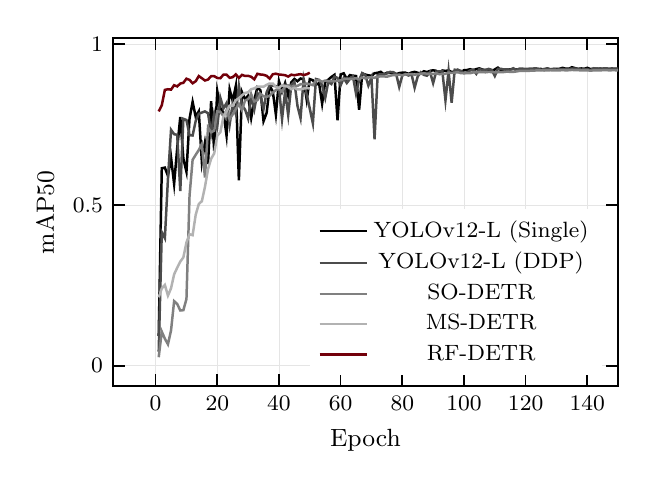
\begin{tikzpicture}
\begin{axis}[
  xlabel={Epoch},
  ylabel={mAP50},
  width=8cm,
  height=6cm,
  xmax=150,
  legend pos=south east,
]

\addplot[linestyle, color=black] coordinates {
  (1,0.092880)
  (2,0.613970)
  (3,0.615930)
  (4,0.590480)
  (5,0.647800)
  (6,0.565330)
  (7,0.676310)
  (8,0.773430)
  (9,0.643890)
  (10,0.603230)
  (11,0.768220)
  (12,0.820120)
  (13,0.773670)
  (14,0.790700)
  (15,0.633410)
  (16,0.693250)
  (17,0.627530)
  (18,0.822720)
  (19,0.668560)
  (20,0.853410)
  (21,0.800540)
  (22,0.786930)
  (23,0.715710)
  (24,0.859330)
  (25,0.822680)
  (26,0.869140)
  (27,0.576660)
  (28,0.850880)
  (29,0.828110)
  (30,0.839380)
  (31,0.770500)
  (32,0.825840)
  (33,0.865260)
  (34,0.855920)
  (35,0.760320)
  (36,0.785880)
  (37,0.868920)
  (38,0.852780)
  (39,0.781090)
  (40,0.884590)
  (41,0.851680)
  (42,0.878480)
  (43,0.840180)
  (44,0.880700)
  (45,0.891500)
  (46,0.884480)
  (47,0.892800)
  (48,0.890630)
  (49,0.826860)
  (50,0.891010)
  (51,0.887410)
  (52,0.873340)
  (53,0.878560)
  (54,0.814970)
  (55,0.882150)
  (56,0.889210)
  (57,0.897640)
  (58,0.904250)
  (59,0.762760)
  (60,0.905420)
  (61,0.909020)
  (62,0.890640)
  (63,0.903380)
  (64,0.901200)
  (65,0.900590)
  (66,0.795560)
  (67,0.908740)
  (68,0.905020)
  (69,0.902790)
  (70,0.901060)
  (71,0.909240)
  (72,0.910640)
  (73,0.913540)
  (74,0.905980)
  (75,0.910890)
  (76,0.910390)
  (77,0.911230)
  (78,0.905490)
  (79,0.909830)
  (80,0.910980)
  (81,0.911010)
  (82,0.907300)
  (83,0.911440)
  (84,0.913450)
  (85,0.910630)
  (86,0.908190)
  (87,0.915350)
  (88,0.912780)
  (89,0.916570)
  (90,0.918400)
  (91,0.916660)
  (92,0.908220)
  (93,0.917750)
  (94,0.916430)
  (95,0.918120)
  (96,0.913030)
  (97,0.914560)
  (98,0.919740)
  (99,0.911850)
  (100,0.918600)
  (101,0.919260)
  (102,0.921750)
  (103,0.918700)
  (104,0.922120)
  (105,0.924400)
  (106,0.920370)
  (107,0.919520)
  (108,0.919990)
  (109,0.914460)
  (110,0.921250)
  (111,0.926610)
  (112,0.918810)
  (113,0.920550)
  (114,0.919870)
  (115,0.921360)
  (116,0.922660)
  (117,0.920770)
  (118,0.919000)
  (119,0.921700)
  (120,0.919920)
  (121,0.920980)
  (122,0.920230)
  (123,0.919910)
  (124,0.922360)
  (125,0.922450)
  (126,0.919150)
  (127,0.924180)
  (128,0.921000)
  (129,0.922430)
  (130,0.923160)
  (131,0.923120)
  (132,0.925950)
  (133,0.923240)
  (134,0.923260)
  (135,0.927680)
  (136,0.925240)
  (137,0.922560)
  (138,0.924080)
  (139,0.922980)
  (140,0.926070)
  (141,0.922230)
  (142,0.923170)
  (143,0.923890)
  (144,0.922500)
  (145,0.923030)
  (146,0.923340)
  (147,0.921960)
  (148,0.922910)
  (149,0.922470)
  (150,0.923090)
};
\addlegendentry{YOLOv12-L (Single)}

\addplot[linestyle, color=Gray30] coordinates {
  (1,0.044300)
  (2,0.415370)
  (3,0.396700)
  (4,0.580890)
  (5,0.733330)
  (6,0.719760)
  (7,0.717960)
  (8,0.543440)
  (9,0.767580)
  (10,0.763950)
  (11,0.716840)
  (12,0.715800)
  (13,0.761020)
  (14,0.782970)
  (15,0.787100)
  (16,0.790680)
  (17,0.785010)
  (18,0.722680)
  (19,0.784500)
  (20,0.744620)
  (21,0.832700)
  (22,0.799740)
  (23,0.816460)
  (24,0.749220)
  (25,0.814310)
  (26,0.782630)
  (27,0.870990)
  (28,0.808930)
  (29,0.796950)
  (30,0.768380)
  (31,0.837870)
  (32,0.796920)
  (33,0.847970)
  (34,0.835550)
  (35,0.798060)
  (36,0.849930)
  (37,0.871910)
  (38,0.870170)
  (39,0.869360)
  (40,0.863510)
  (41,0.766700)
  (42,0.853520)
  (43,0.779140)
  (44,0.873390)
  (45,0.883000)
  (46,0.808300)
  (47,0.769740)
  (48,0.890930)
  (49,0.842480)
  (50,0.799160)
  (51,0.753440)
  (52,0.891200)
  (53,0.888550)
  (54,0.872310)
  (55,0.832350)
  (56,0.882940)
  (57,0.875750)
  (58,0.898530)
  (59,0.894850)
  (60,0.871720)
  (61,0.894020)
  (62,0.878850)
  (63,0.891430)
  (64,0.899290)
  (65,0.845820)
  (66,0.888190)
  (67,0.909460)
  (68,0.903840)
  (69,0.870940)
  (70,0.895710)
  (71,0.704100)
  (72,0.903480)
  (73,0.906020)
  (74,0.905770)
  (75,0.908350)
  (76,0.913210)
  (77,0.912850)
  (78,0.907550)
  (79,0.866750)
  (80,0.902290)
  (81,0.906820)
  (82,0.902270)
  (83,0.905990)
  (84,0.864110)
  (85,0.899350)
  (86,0.912150)
  (87,0.904120)
  (88,0.901670)
  (89,0.913120)
  (90,0.878530)
  (91,0.914300)
  (92,0.915070)
  (93,0.914810)
  (94,0.824930)
  (95,0.916010)
  (96,0.817320)
  (97,0.920160)
  (98,0.919460)
  (99,0.916720)
  (100,0.909390)
  (101,0.911390)
  (102,0.917910)
  (103,0.920020)
  (104,0.907230)
  (105,0.922350)
  (106,0.919070)
  (107,0.919190)
  (108,0.922750)
  (109,0.919770)
  (110,0.900610)
  (111,0.922930)
  (112,0.923020)
  (113,0.920520)
  (114,0.921580)
  (115,0.920070)
  (116,0.924500)
  (117,0.918680)
  (118,0.923530)
  (119,0.923360)
  (120,0.922550)
  (121,0.923200)
  (122,0.923310)
  (123,0.924630)
  (124,0.923520)
  (125,0.919650)
  (126,0.922600)
  (127,0.924030)
  (128,0.921560)
  (129,0.922430)
  (130,0.920280)
  (131,0.921760)
  (132,0.922110)
  (133,0.920940)
  (134,0.921940)
  (135,0.923830)
  (136,0.923390)
  (137,0.923100)
  (138,0.920380)
  (139,0.921930)
  (140,0.922010)
  (141,0.918560)
  (142,0.924580)
  (143,0.922160)
  (144,0.924080)
  (145,0.923860)
  (146,0.924570)
  (147,0.923510)
  (148,0.924140)
  (149,0.923480)
  (150,0.923300)
};
\addlegendentry{YOLOv12-L (DDP)}

\addplot[linestyle, color=Gray50] coordinates {
  (1,0.026740)
  (2,0.106420)
  (3,0.084290)
  (4,0.067080)
  (5,0.109940)
  (6,0.201020)
  (7,0.192390)
  (8,0.172030)
  (9,0.172980)
  (10,0.207680)
  (11,0.528770)
  (12,0.640300)
  (13,0.655710)
  (14,0.670740)
  (15,0.689290)
  (16,0.585370)
  (17,0.740370)
  (18,0.726050)
  (19,0.730630)
  (20,0.790970)
  (21,0.788870)
  (22,0.775960)
  (23,0.793850)
  (24,0.766520)
  (25,0.781420)
  (26,0.797570)
  (27,0.813840)
  (28,0.794350)
  (29,0.824450)
  (30,0.828700)
  (31,0.843550)
  (32,0.821620)
  (33,0.825300)
  (34,0.844880)
  (35,0.837670)
  (36,0.835720)
  (37,0.839320)
  (38,0.849020)
  (39,0.856800)
  (40,0.861210)
  (41,0.851650)
  (42,0.869950)
  (43,0.871510)
  (44,0.866540)
  (45,0.870300)
  (46,0.869830)
  (47,0.875110)
  (48,0.875510)
  (49,0.877280)
  (50,0.875090)
  (51,0.872200)
  (52,0.887350)
  (53,0.887730)
  (54,0.882750)
  (55,0.886530)
  (56,0.884390)
  (57,0.884850)
  (58,0.884220)
  (59,0.885800)
  (60,0.887250)
  (61,0.891200)
  (62,0.892720)
  (63,0.891700)
  (64,0.891540)
  (65,0.893670)
  (66,0.890180)
  (67,0.896310)
  (68,0.893180)
  (69,0.895980)
  (70,0.896410)
  (71,0.895150)
  (72,0.898260)
  (73,0.899650)
  (74,0.899480)
  (75,0.898390)
  (76,0.901140)
  (77,0.903580)
  (78,0.903040)
  (79,0.904960)
  (80,0.903020)
  (81,0.905520)
  (82,0.906000)
  (83,0.906760)
  (84,0.904460)
  (85,0.906420)
  (86,0.907240)
  (87,0.909010)
  (88,0.908000)
  (89,0.906890)
  (90,0.907000)
  (91,0.908970)
  (92,0.906450)
  (93,0.907270)
  (94,0.907590)
  (95,0.911350)
  (96,0.910390)
  (97,0.911270)
  (98,0.912420)
  (99,0.909420)
  (100,0.909940)
  (101,0.909900)
  (102,0.909280)
  (103,0.911820)
  (104,0.911520)
  (105,0.912670)
  (106,0.912820)
  (107,0.912160)
  (108,0.913470)
  (109,0.912690)
  (110,0.912180)
  (111,0.912300)
  (112,0.912660)
  (113,0.913050)
  (114,0.914410)
  (115,0.913370)
  (116,0.913340)
  (117,0.914780)
  (118,0.916450)
  (119,0.916470)
  (120,0.916440)
  (121,0.916830)
  (122,0.917160)
  (123,0.917600)
  (124,0.918400)
  (125,0.918290)
  (126,0.917750)
  (127,0.918000)
  (128,0.918610)
  (129,0.917770)
  (130,0.917870)
  (131,0.918140)
  (132,0.919070)
  (133,0.918110)
  (134,0.918590)
  (135,0.919440)
  (136,0.918980)
  (137,0.918950)
  (138,0.917810)
  (139,0.917880)
  (140,0.918140)
  (141,0.917390)
  (142,0.917920)
  (143,0.918000)
  (144,0.917810)
  (145,0.918790)
  (146,0.919180)
  (147,0.918200)
  (148,0.918530)
  (149,0.918510)
  (150,0.918110)
};
\addlegendentry{SO-DETR}

\addplot[linestyle, color=Gray70] coordinates {
  (1,0.212895)
  (2,0.240756)
  (3,0.251423)
  (4,0.218370)
  (5,0.240891)
  (6,0.284274)
  (7,0.304827)
  (8,0.323837)
  (9,0.336978)
  (10,0.383304)
  (11,0.409012)
  (12,0.406069)
  (13,0.469386)
  (14,0.502586)
  (15,0.511751)
  (16,0.556011)
  (17,0.611272)
  (18,0.643446)
  (19,0.660151)
  (20,0.715515)
  (21,0.725795)
  (22,0.774735)
  (23,0.790611)
  (24,0.808794)
  (25,0.808301)
  (26,0.825436)
  (27,0.831463)
  (28,0.840124)
  (29,0.848046)
  (30,0.849850)
  (31,0.859435)
  (32,0.862186)
  (33,0.867487)
  (34,0.867645)
  (35,0.867207)
  (36,0.873267)
  (37,0.877343)
  (38,0.877268)
  (39,0.865892)
  (40,0.863929)
  (41,0.872283)
  (42,0.869446)
  (43,0.867027)
  (44,0.859530)
  (45,0.863848)
  (46,0.858788)
  (47,0.858940)
  (48,0.861785)
  (49,0.862955)
  (50,0.861994)
};
\addlegendentry{MS-DETR}

\addplot[linestyle, color=Garnet] coordinates {
  (1,0.790735)
  (2,0.809700)
  (3,0.857462)
  (4,0.859582)
  (5,0.858226)
  (6,0.872048)
  (7,0.868305)
  (8,0.877125)
  (9,0.879479)
  (10,0.892335)
  (11,0.888519)
  (12,0.877979)
  (13,0.884259)
  (14,0.900513)
  (15,0.893782)
  (16,0.886578)
  (17,0.889688)
  (18,0.899963)
  (19,0.900052)
  (20,0.894563)
  (21,0.893743)
  (22,0.904928)
  (23,0.904607)
  (24,0.894948)
  (25,0.896863)
  (26,0.905755)
  (27,0.894577)
  (28,0.904207)
  (29,0.900808)
  (30,0.901183)
  (31,0.898198)
  (32,0.890310)
  (33,0.907623)
  (34,0.905255)
  (35,0.904393)
  (36,0.901195)
  (37,0.892384)
  (38,0.906174)
  (39,0.907799)
  (40,0.905208)
  (41,0.904396)
  (42,0.903097)
  (43,0.898866)
  (44,0.904818)
  (45,0.902960)
  (46,0.904930)
  (47,0.906341)
  (48,0.903743)
  (49,0.905931)
  (50,0.910975)
};
\addlegendentry{RF-DETR}

\end{axis}
\end{tikzpicture}
\caption{Training progress comparison: mAP50 across all models over epochs.}
\end{figure}



\end{document}
